% MODIFICA EL CONTENIDO QUE VIENE A CONTINUACIÓN DE ACUERDO A TU TRABAJO

\chapter{Problema del Bandido de $k$-brazos}

%%%%%%%%%%%%%%%%%%%%%%%%%%%%%%%%%%%%%%%%%%%%%%%%%%%%%%%%%%%%%
%%%%%%%%%%%%%%%%%%%%%%%%%%%%%%%%%%%%%%%%%%%%%%%%%%%%%%%%%%%%%
\section{Introducción}

    %\begin{itemize}
    %    \item Breve descripción del problemas y su relevancia.
    %    \item Motivación del trabajo: ¿Por qué es importante el problema estudiado?
    %    \item Objetivos del informe: ¿Qué se pretende lograr con el desarrollo del trabajo?
    %    \item Organización del documento: breve explicación de la estructura del informe.
    %\end{itemize}

    El problema del bandido de $K$ brazos describe un escenario en el cual un agente debe elegir repetidamente entre $k$ opciones diferentes. Al seleccionar una acción, el agente recibe una recompensa numérica proveniente de una distribución de probabilidad desconocida (ej, normal, binomial, bernoulli, etc.) asociada a ese brazo. El objetivo fundamental es maximizar la recompensa total acumulada a lo largo de un número determinado de pasos de tiempo, lo que requiere que el agente aprenda qué acciones son las mejores basándose únicamente en la retroalimentación de sus decisiones previas.

    La importancia y relevancia de este problema reside en su capacidad para modelar el dilema fundamental entre \textbf{exploración} y \textbf{explotación}. Un equilibrio inadecuado entre ambas estrategias resulta costoso, ya que centrarse solo en la explotación puede ignorar la mejor opción de forma permanente, mientras que una exploración excesiva genera un alto arrepentimiento acumulado al desperdiciar recursos en opciones subóptimas. Debido a esta capacidad para optimizar decisiones bajo incertidumbre, el modelo es muy útil y práctico en aplicaciones del mundo real, como pueden ser ensayos clínicos médicos, marketing digital (pruebas A/B), sistemas de recomendación y gestión de redes.

    El objetivo de este informe es analizar y comparar las principales estrategias algorítmicas diseñadas para resolver el problema del bandido multibrazo, desde métodos básicos basados en estimaciones de valor de acción como el algoritmo el $\varepsilon$-\textit{greedy}, hasta enfoques más sofisticados como los métodos de límite superior de confianza (UCB), el ascenso del gradiente y los métodos bayesianos. En última instancia, se busca comprender cómo estas estrategias gestionan el equilibrio exploración-explotación para maximizar la recompensa obtenida en entornos inciertos. 

    El informe se organiza del siguiente modo, la sección de Desarrollo presenta la definición formal del problema, revisa los enfoques existentes en la literatura y describe los métodos implementados. La sección de Algoritmos recoge todos los algoritmos implementados, explicandolos paso a paso y mostrando su pseudocodigo. La sección de Resultados recoge los experimentos realizados y analiza el comportamiento de cada algoritmo. Finalmente, la sección de Conclusiones resume los hallazgos principales.


\section{Desarrollo}
	%\begin{itemize}
        %\item Definición formal del problema o aplicación específica abordada.
        %\item Describir enfoques existentes en la literatura sobre problemas similares.
        %\item Contexto y antecedentes necesarios para entender el trabajo.
        %\item Explicación de los métodos utilizados para abordar el problema.
        %\item Justificar cómo el presente trabajo se diferencia o mejora enfoques previos.
    %\end{itemize}

El bandido de $K$-brazos \cite{robbins1952} es un proceso de decisión secuencial en el que, en cada instante $t = 1,2,\dots,T$, un agente elige una acción $a_t \in \mathcal{A} = \{a_1,\dots,a_k\}$ y recibe una recompensa $r_t \sim p(r \mid a_t)$ proveniente de una distribución desconocida.

\begin{definition}[Valor de una acción]
El valor real de una acción $a$ es la recompensa esperada al seleccionarla: $q(a) = \mathbb{E}[R_t \mid A_t = a]$.
\end{definition}

Como $q(a)$ es desconocido, el agente debe estimarlo a partir de la experiencia. El objetivo es maximizar la recompensa acumulada $\sum_{t=1}^{T} r_t$, lo que equivale a minimizar el \textit{arrepentimiento esperado}:
\begin{equation}
    \mathbb{E}[R_T] = T\,q^* - \sum_{t=1}^{T} \mathbb{E}[r_t], \qquad q^* = \max_{a \in \mathcal{A}} q(a)
\end{equation}
El reto central es el equilibrio entre \textbf{exploración} (probar brazos poco conocidos para mejorar las estimaciones) y \textbf{explotación} (seleccionar el brazo con mayor recompensa esperada conocida).

Desde su formulación, han surgido cuatro grandes familias de soluciones para este problema:

\begin{enumerate}

    \item \textbf{Métodos acción-valor con exploración heurística.} Estiman $q(a)$ como el promedio de recompensas observadas y aplican una política que intercala explotación y exploración. El \textbf{$\varepsilon$-\textit{greedy}} explora al azar con probabilidad fija $\varepsilon$ \cite{sutton2018}, mientras que el \textbf{$\varepsilon$-decaimiento} reduce $\varepsilon$ gradualmente para favorecer la explotación conforme avanza el aprendizaje.

    \item \textbf{Métodos de índice (\textit{Upper Confidence Bound}, UCB).} Seleccionan la acción que maximiza un índice que combina valor estimado e incertidumbre. UCB1 \cite{auer2002} aplica el principio de \textit{optimismo ante la incertidumbre} y garantiza un arrepentimiento acotado por $O(\ln T)$.

    \item \textbf{Métodos de ascenso del gradiente.} Aprenden una preferencia $H_t(a)$ mediante gradiente estocástico y asignan probabilidades de selección mediante una función \textit{softmax} \cite{sutton2018}.

    \item \textbf{Métodos bayesianos.} Mantienen una distribución posterior sobre los parámetros de cada brazo, actualizada con la regla de Bayes. El \textbf{Muestreo de Thompson} \cite{thompson1933, russo2018} muestrea de la posterior y selecciona el brazo con mayor valor estimado, logrando una exploración adaptativa eficaz.

\end{enumerate}

También hay que mencionar una diferencia entre el aprendizaje supervisado, que proporciona \textbf{retroalimentación instructiva} (la acción correcta es conocida), y el bandido multibrazo, el cual opera con \textbf{retroalimentación evaluativa}. En el problema del bandido el agente solo conoce la calidad de la acción tomada, no si existía una mejor \cite{sutton2018}. Además, es un entorno \textbf{no asociativo}, pues el agente no observa ningún estado que condicione su decisión, lo que lo convierte en el modelo más simple del aprendizaje por refuerzo. A lo largo de este trabajo se asume que las distribuciones de recompensa son \textbf{estacionarias} ($p(r \mid a)$ no varía con el tiempo), condición bajo la que los algoritmos presentados ofrecen sus mejores garantías teóricas.

Se han implementado cinco algoritmos que cubren tres de las familias descritas anteriormente. Todos estiman los valores de acción mediante actualización incremental del promedio y se diferencian en su política de selección de brazos, \textbf{$\varepsilon$-Greedy}, que explora aleatoriamente con probabilidad fija $\varepsilon$. \textbf{$\varepsilon$-Greedy con inicialización}, variante que garantiza visitar todos los brazos antes de aplicar la política, corrigiendo el comportamiento incorrecto del greedy puro ($\varepsilon = 0$). \textbf{$\varepsilon$-Decaimiento}, que reduce $\varepsilon$ inversamente proporcional al tiempo para favorecer la explotación conforme avanza el aprendizaje. \textbf{UCB1} \cite{auer2002}, que selecciona el brazo con mayor límite superior de confianza combinando valor estimado e incertidumbre. Y \textbf{Softmax (Gibbs)}, que muestrea acciones según una distribución proporcional a sus valores estimados, controlada por una temperatura $\tau$. Los detalles de cada algoritmo se desarrollan en profundidad en la sección de Algoritmos. Esta selección cubre una progresión natural de complejidad que permite comparar, bajo condiciones experimentales idénticas, estrategias heurísticas simples, el enfoque con garantías teóricas de UCB1 y la política probabilística continua de Softmax.


%%%%%%%%%%%%%%%%%%%%%%%%%%%%%%%%%%%%%%%%%%%%%%%%%%%%%%%%%%%%%
%\subsection{Trabajos Relacionados}

%Por supuesto puede añadir más subapartados si los necesitara.

%%%%%%%%%%%%%%%%%%%%%%%%%%%%%%%%%%%%%%%%%%%%%%%%%%%%%%%%%%%%%
%\subsubsection{Más subsecciones}

%Pero no debería poner más de profundidad tres.

%¡Ah! No olvide poner las correspondientes citas como \cite{ref1, ref2}.



%%%%%%%%%%%%%%%%%%%%%%%%%%%%%%%%%%%%%%%%%%%%%%%%%%%%%%%%%%%%%
%%%%%%%%%%%%%%%%%%%%%%%%%%%%%%%%%%%%%%%%%%%%%%%%%%%%%%%%%%%%%
\section{Algoritmos}
    %\begin{itemize}
        %\item Explicar en detalle los pasos de los algoritmos empleados.
        %\item Incluir pseudocódigo y, opcionalmente, diagramas de flujo si es necesario.
        %\item Justificar la elección de los algoritmos y su aplicabilidad al problema estudiado.
    %\end{itemize}

A continuación se describe en detalle cada uno de los cinco algoritmos. Todos comparten la regla de actualización incremental del promedio (Algoritmo~\ref{algo:update}), que opera en tiempo y espacio $O(1)$ por paso, garantizando condiciones de comparación homogéneas. Los métodos de gradiente y bayesianos, aunque más potentes, quedan fuera del alcance de este trabajo.

\begin{algorithm}
\caption{Actualización incremental del valor estimado}\label{algo:update}
\begin{algorithmic}[1]
\Require Brazo seleccionado $a$, recompensa observada $r$
\State $N(a) \gets N(a) + 1$
\State $Q(a) \gets Q(a) + \dfrac{1}{N(a)}\bigl(r - Q(a)\bigr)$
\end{algorithmic}
\end{algorithm}

\subsection*{$\varepsilon$-Greedy}

Método más simple para incorporar exploración. Con probabilidad $\varepsilon$ selecciona un brazo aleatorio, con probabilidad $1-\varepsilon$ explota el brazo de mayor valor estimado. Los empates se rompen aleatoriamente para evitar sesgo hacia índices bajos. Es el punto de partida natural para entender el dilema exploración-explotación. Nótese que para $\varepsilon=0$ (greedy puro) el agente explota desde el primer paso sin haber visitado todos los brazos, limitación que corrige el algoritmo siguiente. Su simplicidad lo convierte en la linea base a implementar ya que cualquier mejora sobre él cuantifica directamente el beneficio de estrategias más sofisticadas.

\begin{algorithm}
\caption{$\varepsilon$-Greedy}\label{algo:egreedy}
\begin{algorithmic}[1]
\Require $k$ (brazos), $\varepsilon \in [0,1]$
\State $N(a) \gets 0$, $Q(a) \gets 0$ \textbf{para todo} $a$
\For{$t = 1, 2, \dots, T$}
    \If{$\text{Uniforme}(0,1) < \varepsilon$}
        \State $A_t \gets$ brazo aleatorio de $\{1,\dots,k\}$ \Comment{Exploración}
    \Else
        \State $A_t \gets \arg\max_a Q(a)$, empates rotos aleatoriamente \Comment{Explotación}
    \EndIf
    \State Recibir recompensa $R_t$
    \State Actualizar $N(A_t)$ y $Q(A_t)$ (Alg.~\ref{algo:update})
\EndFor
\end{algorithmic}
\end{algorithm}

\subsection*{$\varepsilon$-Greedy con inicialización}

Extiende el anterior añadiendo una fase de arranque que visita todos los brazos al menos una vez antes de aplicar la política. Esto es imprescindible para el caso $\varepsilon=0$ (greedy puro), donde sin inicialización el agente nunca exploraría. Garantiza que $Q(a)$ se basa en al menos una observación real de cada brazo antes de tomar decisiones de explotación, haciendo la comparación con $\epsilon$-Greedy más equitativa.

\begin{algorithm}
\caption{$\varepsilon$-Greedy con inicialización}\label{algo:egreedy_init}
\begin{algorithmic}[1]
\Require $k$, $\varepsilon \in [0,1]$
\State $N(a) \gets 0$, $Q(a) \gets 0$ \textbf{para todo} $a$
\For{$t = 1, 2, \dots, T$}
    \If{$\exists\, a : N(a) = 0$}
        \State $A_t \gets$ brazo aleatorio de $\{a : N(a) = 0\}$ \Comment{Inicialización}
    \EndIf
    \State Igual que Alg.~\ref{algo:egreedy}
\EndFor
\end{algorithmic}
\end{algorithm}

\subsection*{$\varepsilon$-Decaimiento}

Reduce $\varepsilon$ con el tiempo mediante decaimiento inversamente proporcional, de modo que el agente explora ampliamente al inicio y converge hacia la explotación a medida que acumula experiencia. El parámetro $\varepsilon_{\min}$ evita que la exploración se anule por completo. Es el más adecuado para entornos estacionarios con $T$ grande, donde concentrar la exploración al inicio y converger hacia la explotación es la estrategia óptima a largo plazo.

\begin{algorithm}
\caption{$\varepsilon$-Decaimiento}\label{algo:edecay}
\begin{algorithmic}[1]
\Require $k$, $\varepsilon_0$, $\lambda > 0$, $\varepsilon_{\min} \geq 0$
\State $N(a) \gets 0$, $Q(a) \gets 0$ \textbf{para todo} $a$, $t \gets 0$
\For{paso $= 1, 2, \dots, T$}
    \If{$\exists\, a : N(a) = 0$}
        \State $A \gets$ brazo aleatorio de $\{a : N(a) = 0\}$ \Comment{Inicialización}
    \Else
        \State $\varepsilon_t \gets \max\!\left(\varepsilon_{\min},\; \dfrac{\varepsilon_0}{1+\lambda t}\right)$
        \State $A \gets$ selección según Alg.~\ref{algo:egreedy} con $\varepsilon = \varepsilon_t$
    \EndIf
    \State Recibir $R$ y actualizar $N(A)$, $Q(A)$
\EndFor
\end{algorithmic}
\end{algorithm}

\subsection*{UCB1}

Aplica el principio de \textit{optimismo ante la incertidumbre}, selecciona el brazo con mayor límite superior de confianza, que combina el valor estimado con un bonus que decrece conforme el brazo es más explorado. No requiere hiperparámetro de exploración aleatorio ya que $c$ controla únicamente la amplitud del intervalo de confianza. Es el único algoritmo del conjunto con garantías teóricas de regret sublineal ($O(k \ln T)$), lo que justifica su inclusión como cota de referencia para los métodos heurísticos.

\begin{algorithm}
\caption{UCB1}\label{algo:ucb1}
\begin{algorithmic}[1]
\Require $k$, $c \geq 0$
\State $N(a) \gets 0$, $Q(a) \gets 0$ \textbf{para todo} $a$
\For{$t = 1, 2, \dots, T$}
    \If{$\exists\, a : N(a) = 0$}
        \State $A_t \gets$ brazo aleatorio de $\{a : N(a) = 0\}$ \Comment{Fase inicial aleatoria}
    \Else
        \State $t_{\text{total}} \gets \sum_a N(a)$
        \State $A_t \gets \arg\max_{a}\!\left[ Q(a) + c\sqrt{\dfrac{\ln t_{\text{total}}}{N(a)}} \right]$
    \EndIf
    \State Recibir $R_t$ y actualizar $N(A_t)$, $Q(A_t)$
\EndFor
\end{algorithmic}
\end{algorithm}

\subsection*{Softmax (Gibbs)}

En lugar de una política binaria explorar/explotar, asigna a cada brazo una probabilidad de selección proporcional a su valor estimado mediante la función de Gibbs. La temperatura $\tau$ regula la concentración de la distribución, donde $\tau \to 0$ equivale a la política greedy, mientras que $\tau \to \infty$ produce una selección uniforme aleatoria. Para prevenir desbordamientos numéricos, se sustrae el máximo de los valores antes de calcular las exponenciales. Resulta especialmente adecuado cuando las diferencias de valor entre brazos son pequeñas, ya que la política probabilística continua evita descartar prematuramente brazos cuyas estimaciones estén próximas al óptimo.

\begin{algorithm}
\caption{Softmax (Gibbs)}\label{algo:softmax}
\begin{algorithmic}[1]
\Require $k$, $\tau > 0$
\State $N(a) \gets 0$, $Q(a) \gets 0$ \textbf{para todo} $a$
\For{$t = 1, 2, \dots, T$}
    \State $Q_{\max} \gets \max_a Q(a)$
    \State $\pi(a) \gets \dfrac{\exp\!\left(\dfrac{Q(a)-Q_{\max}}{\tau}\right)}
                               {\sum_{b=1}^{k}\exp\!\left(\dfrac{Q(b)-Q_{\max}}{\tau}\right)}$
           \textbf{para todo} $a$
    \State $A_t \gets$ brazo aleatorio con probabilidades $\pi$
    \State Recibir $R_t$ y actualizar $N(A_t)$, $Q(A_t)$
\EndFor
\end{algorithmic}
\end{algorithm}

%%%%%%%%%%%%%%%%%%%%%%%%%%%%%%%%%%%%%%%%%%%%%%%%%%%%%%%%%%%%%
%%%%%%%%%%%%%%%%%%%%%%%%%%%%%%%%%%%%%%%%%%%%%%%%%%%%%%%%%%%%%
\section{Evaluación/Experimentos}
    %\begin{itemize}
    %    \item Configuración experimental: herramientas, entornos de prueba, datasets empleados, etc.
    %    \item Métricas utilizadas para evaluar el desempeño del método propuesto.
    %    \item Resultados obtenidos, presentados en tablas o gráficos según corresponda.
    %    \item Análisis crítico de los resultados y comparación con otros enfoques.
    %\end{itemize}

\subsection*{Configuración experimental}

Los experimentos se han implementado en Python y Jupyter Notebooks como entorno de ejecución. Se han evaluado los cinco algoritmos en \textbf{tres entornos de distribución} distintos con $k=10$ brazos, $T=1000$ pasos (excepto UCB1, con $T=500$ por su convergencia más rápida) y 500 ejecuciones independientes, con semilla fija (\texttt{seed = 42}) para reproducibilidad. Los rangos de hiperparámetros explorados han sido: $\varepsilon \in \{0,\, 0{.}01,\, 0{.}1,\, 0{.}2\}$ para $\varepsilon$-Greedy. $\lambda \in \{0{.}001,\, 0{.}01,\, 0{.}1\}$ y $\varepsilon_{\min} \in \{0,\, 0{.}1\}$ para $\varepsilon$-Decaimiento. $c \in \{0{.}1,\, 0{.}5,\, 1,\, 2,\, 5\}$ para UCB1. $\tau \in \{0{.}1,\, 0{.}5,\, 1,\, 2,\, 5\}$ para Softmax. La comparación final entre algoritmos usa $\varepsilon{=}0{.}1$, $\lambda{=}0{.}001$/$\varepsilon_{\min}{=}0{.}1$, $c{=}1$ y $\tau{=}1$ en los entornos Normal y Binomial. en Bernoulli se ajustan a $c{=}0{.}5$ y $\tau{=}0{.}1$ por el comportamiento diferencial observado en ese entorno.

Adicionalmente, se realiza un estudio específico sobre el efecto de la fase de inicialización, comparando $\varepsilon$-Greedy estándar frente a $\varepsilon$-Greedy con inicialización para $\varepsilon \in \{0,\, 0{.}01,\, 0{.}1\}$ sobre el entorno Normal ($T=1000$, 500 ejecuciones). Las distribuciones de probabilidad han sido las siguientes:

\begin{itemize}
    \item \textbf{Normal} $\mathcal{N}(\mu, \sigma^2)$: medias $\mu_i$ muestreadas uniformemente en $[1, 10]$ con $\sigma = 1{.}0$. Es el entorno de referencia, con alta señal y varianza moderada.

    \item \textbf{Bernoulli} $\text{Bern}(p)$: probabilidades $p_i$ muestreadas en $[0{.}1,\, 0{.}9]$. Recompensas binarias $\{0, 1\}$, esto conlleva mayor dificultad de discriminación por la baja varianza informativa por tirada.

    \item \textbf{Binomial} $\text{Bin}(n{=}10,\, p)$: probabilidades en $[0{.}1,\, 0{.}9]$, valor esperado $\mu_i = n p_i \in [1, 9]$. Amplifica la señal Bernoulli manteniendo la misma estructura estocástica.
\end{itemize}

\subsection*{Métricas de evaluación}

Se emplean cuatro métricas complementarias para caracterizar el comportamiento de cada algoritmo:

\begin{enumerate}

    \item \textbf{Recompensa promedio} ($\bar{r}_t$). Media de las recompensas obtenidas en el paso $t$ sobre todos los episodios. Refleja la velocidad de aprendizaje y el nivel de explotación alcanzado. Un algoritmo ideal converge rápidamente hacia $q^* = \max_a q(a)$.

    \item \textbf{Porcentaje de selecciones óptimas} (\% opt.). Fracción de pasos en que el agente elige el brazo con mayor recompensa esperada, promediada sobre episodios. Mide directamente la calidad de la política aprendida, independientemente de la escala de las recompensas.

    \item \textbf{Arrepentimiento acumulado} ($R_T$). Diferencia entre la recompensa del agente óptimo y la del algoritmo: $R_T = T\,q^* - \sum_{t=1}^{T} r_t$. Se contrasta con la cota asintótica de Lai y Robbins \cite{lai1985}, calculada a partir de la divergencia KL entre cada brazo subóptimo y el óptimo, que establece el crecimiento mínimo $\Theta(\ln T)$ de cualquier algoritmo consistente. Es la métrica más informativa de las empleadas, pues integra toda la historia de decisiones y permite comparar algoritmos independientemente de la escala de recompensas.

    %Diferencia entre la recompensa total obtenida por el agente óptimo y la del algoritmo evaluado:
    %\begin{equation}
    %    R_T = T\,q^* - \sum_{t=1}^{T} r_t
    %\end{equation}
    %Se compara con la \textbf{cota asintótica de Lai y Robbins} \cite{lai1985}, que
    %establece que todo algoritmo consistente satisface:
    %\begin{equation}
    %    \liminf_{T\to\infty} \frac{\mathbb{E}[R_T]}{\ln T}
    %    \;\geq\; \sum_{i:\,\mu_i < \mu^*} \frac{\mu^* - \mu_i}{I(\mu_i,\,\mu^*)}
    %\end{equation}
    %donde $I(\mu_i, \mu^*)$ es la divergencia de Kullback-Leibler entre la distribución
    %del brazo $i$ y la del brazo óptimo. Para los tres entornos empleados:
    %\begin{itemize}
    %    \item Normal: $I(\mu_i, \mu^*) = (\mu^* - \mu_i)^2 / (2\sigma^2)$
    %    \item Bernoulli/Binomial: $I(p_i, p^*) = n\left[p_i \ln\tfrac{p_i}{p^*}
    %          + (1-p_i)\ln\tfrac{1-p_i}{1-p^*}\right]$
    %\end{itemize}
    %Esta cota proporciona una referencia teórica con la que contrastar el arrepentimiento empírico de cada algoritmo.

    \item \textbf{Estadísticas de brazos.} Para cada algoritmo se visualiza, por brazo, la recompensa promedio observada y el número de selecciones acumuladas (indicado en la etiqueta del eje X). Las barras se colorean distinguiendo el brazo óptimo (verde), los subóptimos (azul) y los no visitados (gris), una línea discontinua roja marca el valor de recompensa del brazo óptimo como referencia. Permite detectar si el algoritmo concentra correctamente las selecciones en el brazo óptimo o desperdicia tiradas en brazos claramente inferiores.

\end{enumerate}

\subsection*{Resultados}

\subsubsection*{$\varepsilon$-Greedy y $\varepsilon$-Greedy con inicialización}

Sin inicialización, $\varepsilon{=}0$ produce un regret lineal (${\approx}4000$ a $T{=}1000$) al quedar atrapado en el primer brazo explotado. $\varepsilon{=}0{.}1$ es el mejor (${\approx}580$), aunque todos superan ampliamente la cota teórica (${\approx}50$). Pero al aplicar la inicialización invierte completamente el ranking, ahora $\varepsilon{=}0$ y $\varepsilon{=}0{.}01$ pasan a ser los mejores (${\approx}145$), pues identifican el óptimo durante la fase de arranque y lo explotan sin desperdicio, y $\varepsilon{=}0{.}1$ se convierte en el peor (${\approx}460$) porque su exploración continua genera regret innecesario una vez que todos los brazos ya han sido visitados. En conjunto, la inicialización reduce el regret máximo en un orden de magnitud.

\begin{table}[h]
    \centering
    \small
    \begin{tabular}{lccc}
        \toprule
        & $\varepsilon{=}0$ & $\varepsilon{=}0{.}01$ & $\varepsilon{=}0{.}1$ \\
        \midrule
        Sin inicialización & 4050 & 1340 & \textbf{580} \\
        Con inicialización & \textbf{145} & \textbf{145} & 460 \\
        \bottomrule
    \end{tabular}
    \caption{Regret acumulado a $T{=}1000$ para $\varepsilon$-Greedy con y sin
    inicialización. En negrita, la mejor configuración de cada variante.}
    \label{tab:greedy_init}
\end{table}

\subsubsection*{Distribución normal}

UCB1 es el único algoritmo que se aproxima a la cota de Lai-Robbins ($k{=}10$, $T{=}1000$, UCB1 con $T{=}500$), su bono $c\sqrt{\ln t / N_i}$ dirige la exploración hacia los brazos con mayor incertidumbre, logrando regret sublineal. Softmax ($\tau{=}1$) es el peor (${\approx}1250$) porque esa temperatura aplana la distribución de selección sobre la escala $\mu_i \in [1,10]$, comportándose como exploración casi uniforme. $\varepsilon$-Decaimiento produce regret lineal acotado por el piso $\varepsilon_{\min}{=}0{.}1$, incluso con $\lambda$ alto. Frente a Thompson Sampling, UCB1 es más robusto al no requerir distribución a priori, aunque su rendimiento depende del ajuste de $c$.

\begin{table}[h]
    \centering
    \small
    \begin{tabular}{lcc}
        \toprule
        Algoritmo & Mejor config. & Regret \\
        \midrule
        $\varepsilon$-Greedy      & $\varepsilon{=}0{.}1$   & 560 \\
        $\varepsilon$-Decaimiento & $\lambda{=}0{.}1$       & 530 \\
        UCB1                      & $c{=}1$                 & \textbf{50}$^\dagger$ \\
        Softmax                   & $\tau{=}1$              & 1250 \\
        \midrule
        Cota teórica              & ---                     & ${\approx}50$ \\
        \bottomrule
    \end{tabular}
    \caption{Mejor configuración de cada algoritmo en distribución normal.
    $^\dagger$Medido a $T{=}500$. En negrita, el mejor resultado.}
    \label{tab:normal_best}
\end{table}

\begin{figure}[h]
    \centering
    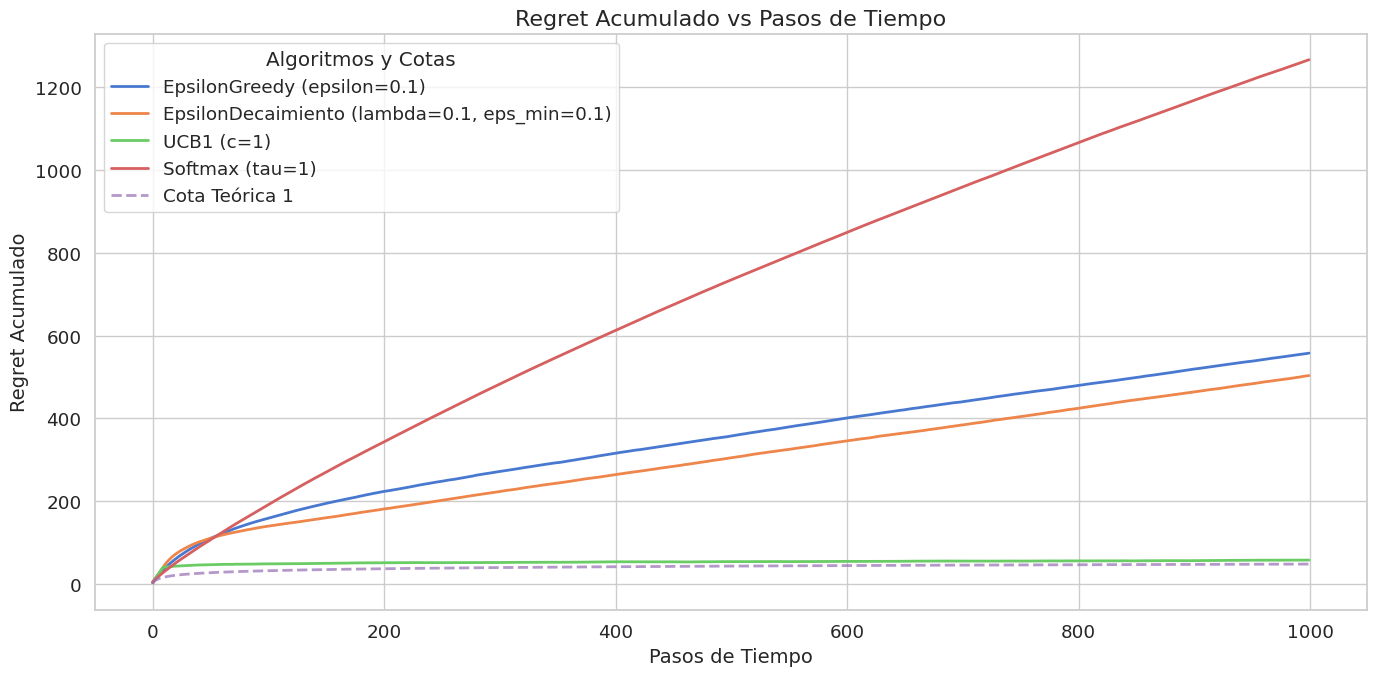
\includegraphics[width=\linewidth]{imagenes/Normal-regret-general-mejores-parametros.png}
    \caption{Regret acumulado en distribución normal para la mejor configuración
    de cada algoritmo. UCB1 ($c{=}1$) se aproxima a la cota teórica; el resto
    exhiben regret lineal o sublineal pero alejado del óptimo.}
    \label{fig:normal_general}
\end{figure}

\subsubsection*{Distribución binomial}

La distribución binomial ($B(10,p_i)$, $k{=}10$, $T{=}1000$, UCB1 con $T{=}500$) reproduce el patrón anterior con UCB1 dominante, pero la cota teórica es mayor (${\approx}90$) porque la KL entre binomiales es menor que entre normales para el mismo $\Delta$, lo que requiere más muestras para descartar brazos subóptimos. Softmax ($\tau{=}1$) vuelve a ser el peor, las recompensas enteras en $\{0,\ldots,10\}$ generan selección casi uniforme para esa temperatura. $\varepsilon$-Decaimiento mejora levemente a $\varepsilon$-Greedy gracias a la reducción progresiva de exploración, pero ambos exhiben regret lineal lejos del óptimo logarítmico.

\begin{table}[h]
    \centering
    \small
    \begin{tabular}{lcc}
        \toprule
        Algoritmo & Mejor config. & Regret \\
        \midrule
        $\varepsilon$-Greedy      & $\varepsilon{=}0{.}1$   & 550 \\
        $\varepsilon$-Decaimiento & $\lambda{=}0{.}1$       & 480 \\
        UCB1                      & $c{=}1$                 & \textbf{60}$^\dagger$ \\
        Softmax                   & $\tau{=}1$              & 1000 \\
        \midrule
        Cota teórica              & ---                     & ${\approx}90$ \\
        \bottomrule
    \end{tabular}
    \caption{Mejor configuración de cada algoritmo en distribución binomial.
    $^\dagger$Medido a $T{=}500$. En negrita, el mejor resultado.}
    \label{tab:binomial_best}
\end{table}

\begin{figure}[h]
    \centering
    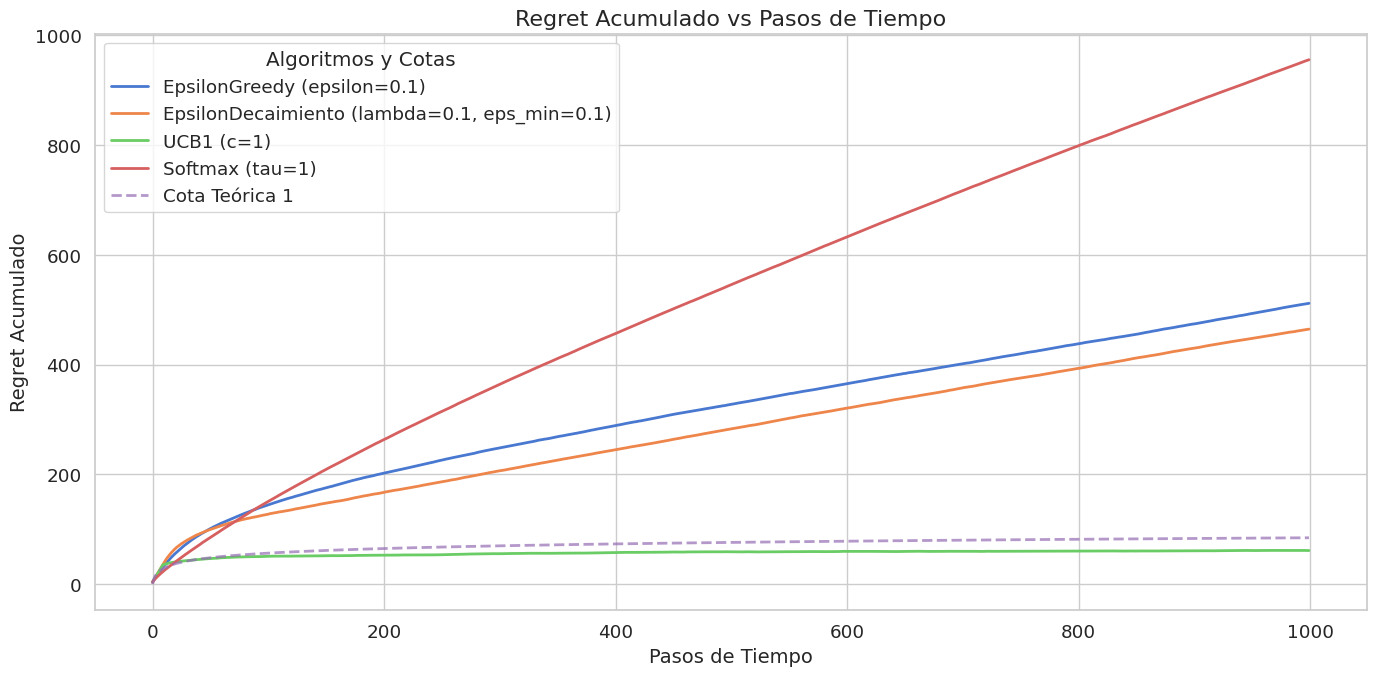
\includegraphics[width=\linewidth]{imagenes/Binomial-regret-general-mejores-parametros.png}
    \caption{Regret acumulado en distribución binomial para la mejor configuración
    de cada algoritmo.}
    \label{fig:binomial_general}
\end{figure}

\subsubsection*{Distribución Bernoulli}

La distribución Bernoulli ($\text{Bern}(p_i)$, $k{=}10$, $T{=}1000$, UCB1 con $T{=}500$) introduce un cambio cualitativo respecto a Normal y Binomial, al estar las recompensas en $\{0,1\}$, los algoritmos necesitan bonos de exploración y temperaturas más pequeñas. UCB1 con $c{=}0{.}1$ logra el mejor resultado (${\approx}25$), muy por debajo de la cota teórica (${\approx}75$), mientras que Softmax invierte su ranking habitual, ahora $\tau{=}0{.}1$ es el mejor (${\approx}100$) porque concentra eficazmente las selecciones en el brazo con mayor $\hat{p}$ estimada. $\varepsilon$-Greedy y $\varepsilon$-Decaimiento se aproximan a la cota teórica con sus mejores configuraciones.

\begin{table}[h]
    \centering
    \small
    \begin{tabular}{lcc}
        \toprule
        Algoritmo & Mejor config. & Regret \\
        \midrule
        $\varepsilon$-Greedy      & $\varepsilon{=}0{.}1$   & 70 \\
        $\varepsilon$-Decaimiento & $\lambda{=}0{.}1$       & 67 \\
        UCB1                      & $c{=}0{.}1$             & \textbf{25}$^\dagger$ \\
        Softmax                   & $\tau{=}0{.}1$          & 100 \\
        \midrule
        Cota teórica              & ---                     & ${\approx}85$ \\
        \bottomrule
    \end{tabular}
    \caption{Mejor configuración de cada algoritmo en distribución Bernoulli.
    $^\dagger$Medido a $T{=}500$. En negrita, el mejor resultado.}
    \label{tab:bernoulli_best}
\end{table}

\begin{figure}[h]
    \centering
    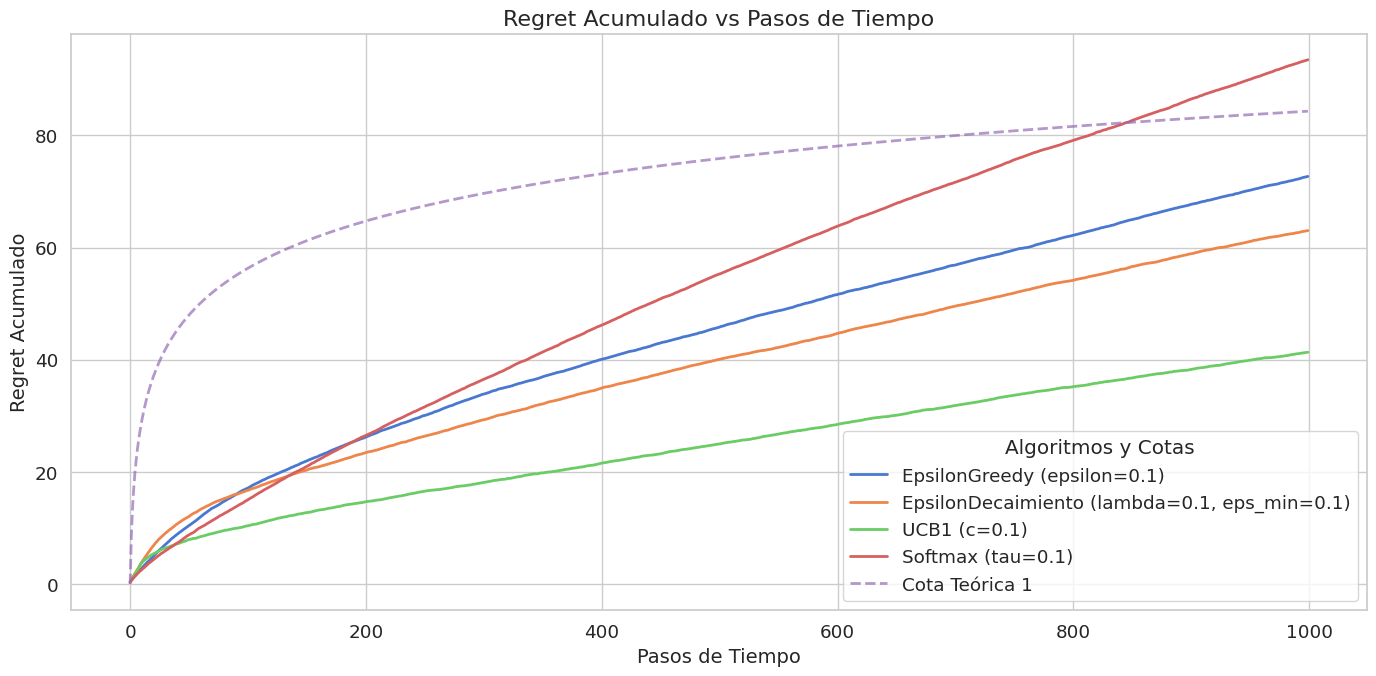
\includegraphics[width=\linewidth]{imagenes/Bernoulli-regret-general-mejores-parametros.png}
    \caption{Regret acumulado en distribución Bernoulli para la mejor configuración
    de cada algoritmo.}
    \label{fig:bernoulli_general}
\end{figure}


%%%%%%%%%%%%%%%%%%%%%%%%%%%%%%%%%%%%%%%%%%%%%%%%%%%%%%%%%%%%%
%%%%%%%%%%%%%%%%%%%%%%%%%%%%%%%%%%%%%%%%%%%%%%%%%%%%%%%%%%%%%   
\section{Conclusiones}
    %\begin{itemize}
    %    \item Un resumen de los principales resultados obtenidos.
    %    \item Limitaciones del estudio y posibles mejoras futuras.
    %    \item Reflexión sobre la importancia del trabajo y su impacto en el campo del aprendizaje por refuerzo.
    %    \item Líneas \textit{futuras} de estudio.
    %\end{itemize}

\textbf{UCB1 es el algoritmo más eficaz en las tres distribuciones estudiadas.} Es el único que logra regret sublineal próximo a la cota de Lai-Robbins, gracias a que su bono de confianza $c\sqrt{\ln t / N_i}$ equilibra exploración y explotación de forma adaptativa. Su parámetro óptimo depende de la escala de recompensas, $c{=}1$ para Normal y Binomial, $c{=}0{.}1$ para Bernoulli, donde las recompensas en $\{0,1\}$ requieren bonos más pequeños.

\textbf{La inicialización optimista transforma $\varepsilon$-Greedy.} Sin inicialización, el ranking es $\varepsilon{=}0{.}1 \succ \varepsilon{=}0{.}01 \succ \varepsilon{=}0$. con inicialización, se invierte: $\varepsilon{=}0$ y $\varepsilon{=}0{.}01$ pasan a ser los mejores (${\approx}145$) porque la fase de arranque forzado ya cubre la exploración necesaria. Es una heurística eficaz pero frágil, ya que requiere conocer la escala de recompensas de antemano.

\textbf{Softmax es el algoritmo más sensible a la distribución.} Su temperatura óptima es $\tau{=}1$ en Normal y Binomial, pero $\tau{=}0{.}1$ en Bernoulli. Un valor inadecuado produce exploración casi uniforme (regret lineal elevado), lo que lo convierte en el más difícil de ajustar en la práctica.

\textbf{La gráfica más relevante es el regret acumulado con cota teórica} (\texttt{plot\_regret}). Es la única que permite:
\begin{itemize}
    \item Cuantificar el coste de oportunidad real de cada algoritmo a lo largo del tiempo.
    \item Comparar directamente con la cota asintótica de Lai-Robbins, determinando si el algoritmo es óptimo en orden de magnitud.
    \item Distinguir regret sublineal ($O(\ln T)$) de lineal ($O(T)$), diferencia cualitativa invisible en \texttt{plot\_average\_rewards}.
\end{itemize}

\texttt{plot\_optimal\_selections} es complementaria, confirmando si la convergencia al brazo óptimo es consistente o puntual. \texttt{plot\_arm\_statistics} resulta útil para diagnóstico (detectar brazos ignorados) pero no para comparar algoritmos. \texttt{plot\_average\_rewards} aporta la menor información diferencial, al no referenciar el óptimo teórico.

\textbf{Limitaciones y líneas futuras.}
Los experimentos se limitan a $k{=}10$ y $T{\leq}1000$, con un único conjunto de brazos por distribución. Ampliar a horizontes mayores y múltiples instancias aleatorias (análisis de varianza del regret) daría resultados más robustos. Como extensión natural, Thompson Sampling y KL-UCB proporcionarían cotas más ajustadas para Bernoulli y Binomial, aprovechando la estructura discreta de sus distribuciones.

